\documentclass[twocolumn, aps, superscriptaddress]{revtex4}
%\documentclass[reprint, prl, aps, showpacs]{revtex4-1}
%\documentclass[preprint, aps, showpacs]{revtex4-1}

\usepackage{graphicx}
\usepackage{amsmath,amssymb}
%\usepackage[usenames,dvipsnames]{color}
%\usepackage[colorlinks=true, citecolor=blue, linkcolor=WildStrawberry]{hyperref}
%\usepackage[citecolor=blue]{hyperref}
%\usepackage[justification=centerfirst]{caption}
\usepackage{epstopdf}

%\usepackage[latin1]{inputenc}
\usepackage{tikz}
\usetikzlibrary{shapes,arrows}

\newcommand{\braket}[2]{\left\langle#1\, |\,#2\,\right\rangle}  %  < #1 | #2 >
\newcommand{\expec}[1]{\langle#1\rangle}  %  < #1 >
\newcommand{\drm}{{\rm d}}
\newcommand{\irm}{{\rm i}}
\newcommand{\beq}{\begin{equation}}
\newcommand{\eeq}{\end{equation}}
\newcommand{\bdm}{\begin{displaymath}}
\newcommand{\edm}{\end{displaymath}}
\newcommand{\T}[1]{\tilde{#1}}
\newcommand{\wT}[1]{\widetilde{#1}}
\newcommand{\Cdot}{\!\cdot\!}
\newcommand{\SNR}{\textnormal{SNR}}
\newcommand{\rednote}[1]{{\color{red} (#1)}}
\newcommand{\fixme}[1]{\textcolor{green}{\textbf{\textit{{#1}}}}}

\DeclareFontFamily{OT1}{pzc}{}
\DeclareFontShape{OT1}{pzc}{m}{it}{<-> s * [1.10] pzcmi7t}{}
\DeclareMathAlphabet{\mathpzc}{OT1}{pzc}{m}{it}

\def\dblone{\hbox{$1\hskip -1.2pt\vrule depth 0pt height 1.6ex width 0.7pt \vrule depth 0pt height 0.3pt width 0.12em$}}

\graphicspath{{./plots/}}
\begin{document}

\title{Limiting the effects of earthquakes on gravitational-wave interferometers}

\author{Michael Coughlin}
\affiliation{Department of Physics, Harvard University, Cambridge, MA 02138, USA}

\author{Nicolas Arnaud}
\affiliation{LAL, Univ. Paris-Sud, CNRS/IN2P3, Universit\'e Paris-Saclay, F-91898 Orsay, France}
\affiliation{European Gravitational Observatory (EGO), I-56021 Cascina, Pisa, Italy}

\author{David Barker}
\affiliation{LIGO Hanford Observatory, Richland, WA 99352, USA}

\author{Sebastien Biscans}
\affiliation{LIGO Laboratory, Massachusetts Institute of Technology, Cambridge, MA 02138, USA}

\author{Christopher Buchanan}
\affiliation{Department of Physics and Astronomy, Louisiana State University, Baton Rouge, LA 70803-4001, USA}

\author{Eric Coughlin}
\affiliation{Department of Computer Science, Luther College, 700 College Dr, Decorah, IA 52101, USA}

\author{Fred Donovan}
\affiliation{LIGO Laboratory, Massachusetts Institute of Technology, Cambridge, MA 02138, USA}

\author{Paul Earle}
\affiliation{U.S. Geological Survey, Golden, CO 80401, USA}

\author{Jeremy Fee}
\affiliation{United States Geological Survey, Golden, CO 80401, USA}

\author{Irene Fiori}
\affiliation{European Gravitational Observatory (EGO), I-56021 Cascina, Pisa, Italy}

\author{Hunter Gabbard}
\affiliation{Albert-Einstein-Institut, Max-Planck-Institut f{\"u}r Gravitationsphysik, D-30167 Hannover, Germany}

\author{Michelle Guy}
\affiliation{United States Geological Survey, Golden, CO 80401, USA}

\author{Jan Harms}
\affiliation{INFN, Sezione di Firenze, Sesto Fiorentino, 50019, Italy\\
Universit\`a degli Studi di Urbino ``Carlo Bo'', I-61029 Urbino, Italy}

\author{Nikhil Mukund}
\affiliation{Inter-University Centre for Astronomy and Astrophysics (IUCAA), Post Bag 4, Ganeshkhind,  Pune 411 007, India}

\author{Matthew Perry}
\affiliation{Planetary Science Institute, Lakewood, CO 80401, USA}

\author{Hugh Radkins}
\affiliation{LIGO Hanford Observatory, Richland, WA 99352, USA}

\author{Bas Swinkels}
\affiliation{European Gravitational Observatory (EGO), I-56021 Cascina, Pisa, Italy}

\author{Keith Thorne}
\affiliation{LIGO Livingston Observatory, Livingston, LA 70754, USA}

\author{Jim Warner}
\affiliation{LIGO Hanford Observatory, Richland, WA 99352, USA}


\begin{abstract}

\end{abstract}

\maketitle

\section{Introduction}
\label{sec:Intro}

With the advent of gravitational-wave astronomy, it is essential to maximize the duty cycle of second generation gravitational-wave detectors such as the Laser Interferometer Gravitational-wave Observatory (LIGO) \cite{aligo}, Virgo \cite{avirgo}, and GEO600 \cite{Gr2010} detectors.
Any increase in duty cycle increases the sensitivity of gravitational-wave searches, including the observations of binary black hole mergers \cite{AbEA2016a,AbEA2016e}.
One source of ground motion that destabilizes the detectors are earthquakes
\cite{CoSt2015,CoEa2017}, despite seismic isolation systems designed to minimize such effects \cite{AbAd2002,StAb2009,MaLa2015}.

In previous work \cite{CoEa2017}, Coughlin et al. used advances in early earthquake warning \cite{Al2012,KuAl2013a,KuAl2013b,KuHe2014,CoLa2009a,CoLa2009b,BoAl2014,HoKa2008,HoEA2011c,StAl2016} to develop a low-latency earthquake early warning client named \emph{Seismon}, which uses a real-time event messaging system of the U.S. Geological Survey (USGS) to mitigate the effects of teleseismic events on ground-based gravitational-wave detectors. 
Using information about the earthquake source characteristics such as time, location, depth, and magnitude, predictions as to the arrival time and ground velocity induced by the earthquakes were predicted.
We showed that about 90\% of events had a measured ground velocity within a factor of 5 of the predicted value.

In this analysis, we leverage the power of machine learning algorithms to improve both the ground velocity predictions as well as the lockloss predictions of \emph{Seismon}. We demonstrate an improvement from a factor of 5 to a factor of 3 in scatter of the error in the predicted ground velocity.

In section~\ref{sec:algorithm}, we describe recent improvements to the algorithm.
In section~\ref{sec:performance}, we describe a case-study on a recent earthquake to demonstrate the benefits of low-latency earthquake notification as well as the challenges that still lie ahead.
In section~\ref{sec:conclusions}, we offer concluding remarks and suggest directions for future research.

\section{Algorithm}
\label{sec:algorithm}

\subsection{Ground Velocity Prediction Performance}

\begin{figure*}[t]
\hspace*{-0.5cm}
 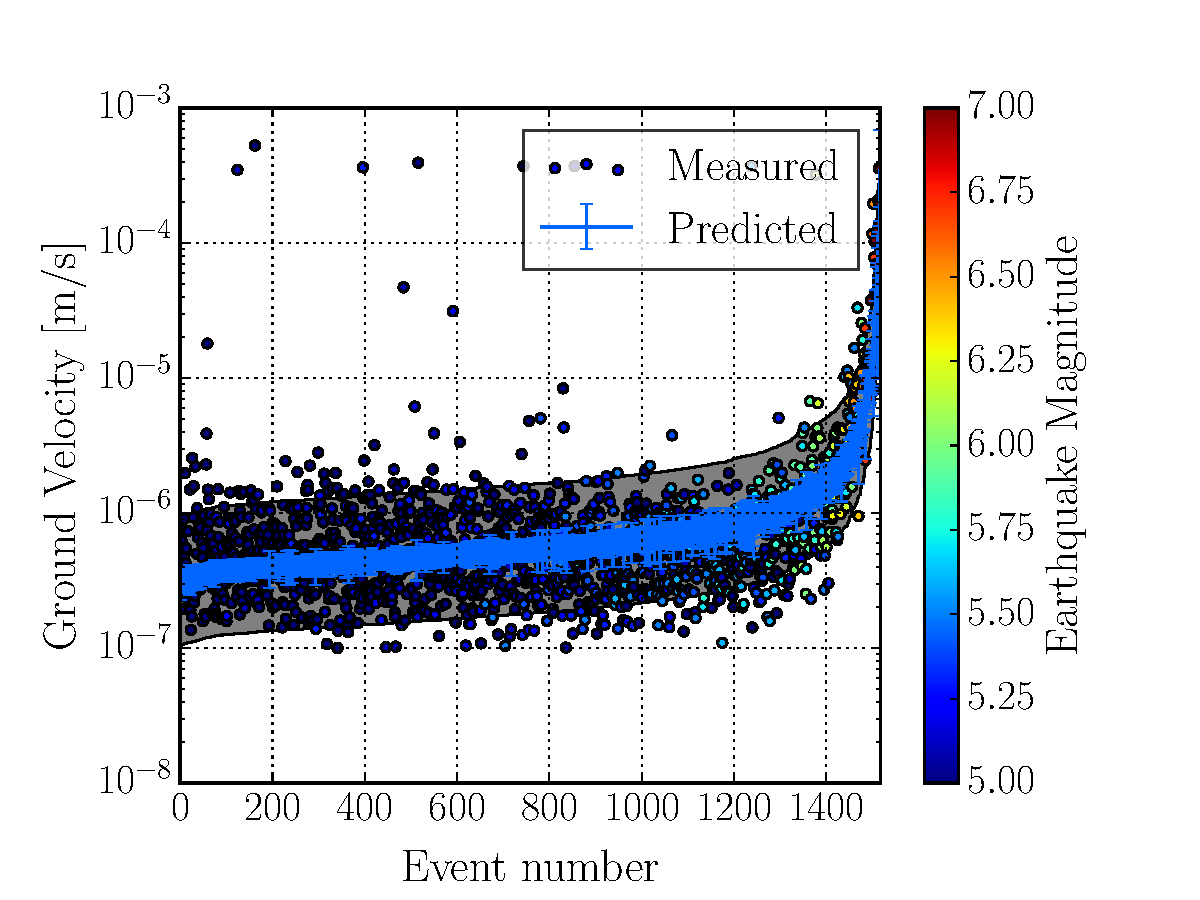
\includegraphics[width=3.5in,trim = 2.5cm 1.5cm 2.5cm 1.5cm, clip=true]{prediction_H1O1O2_GPR.pdf}
 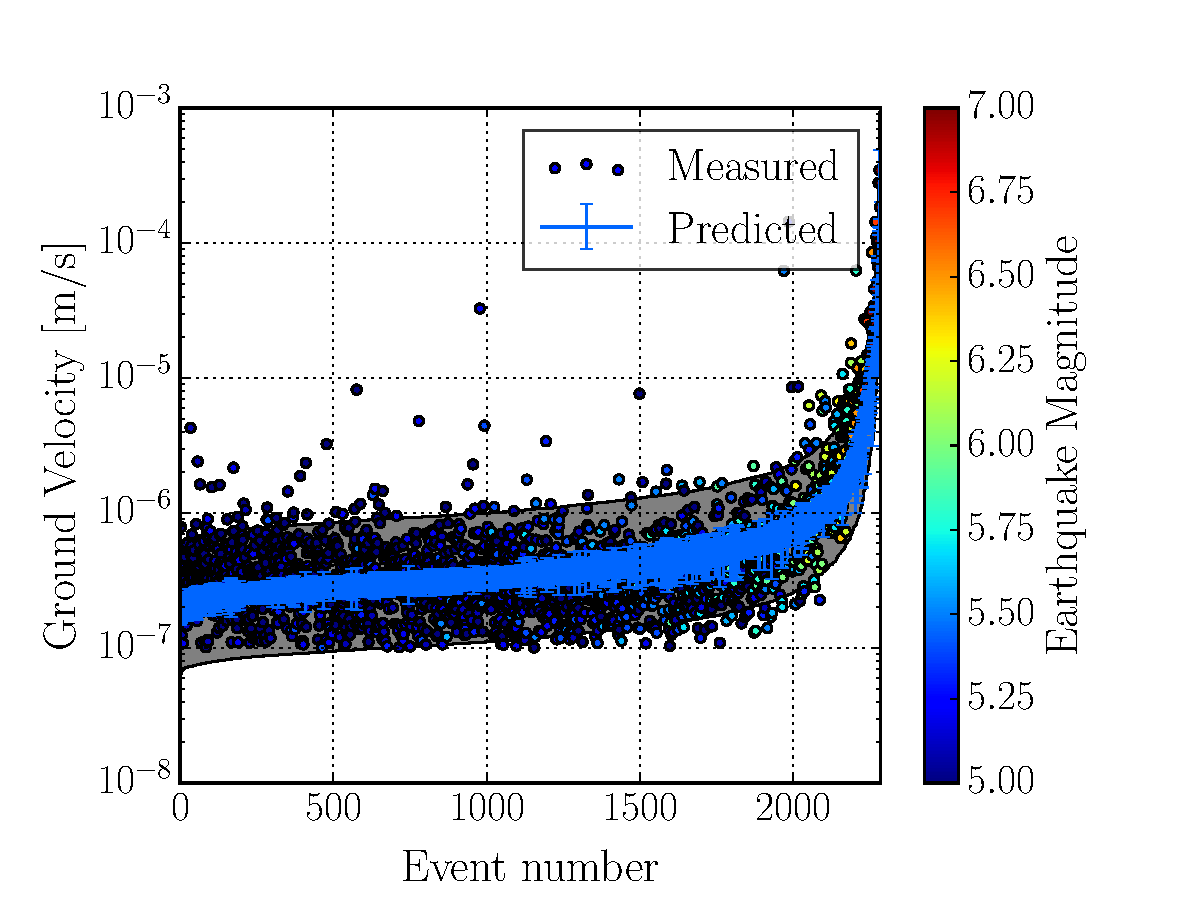
\includegraphics[width=3.5in,trim = 2.5cm 1.5cm 2.5cm 1.5cm, clip=true]{prediction_L1O1O2_GPR.pdf}
 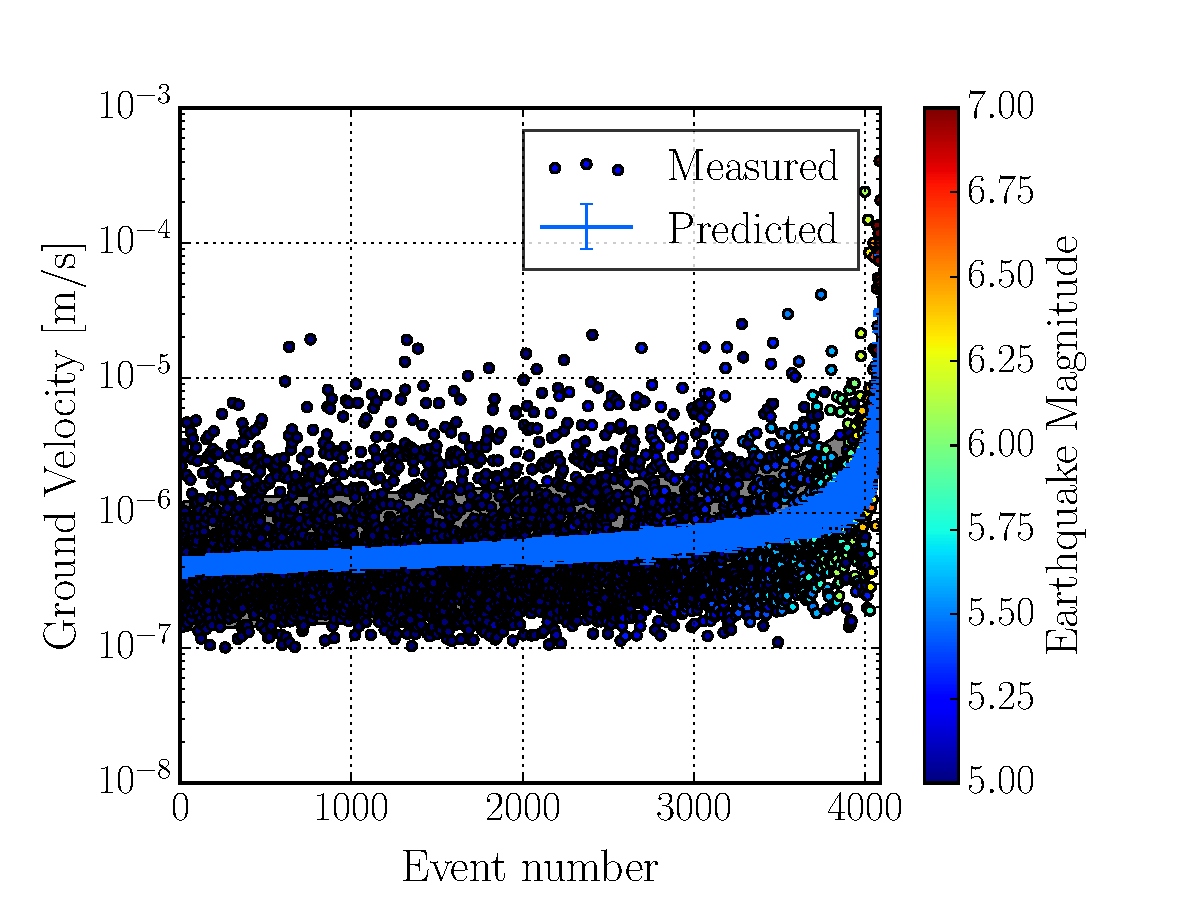
\includegraphics[width=3.5in,trim = 2.5cm 1.5cm 2.5cm 1.5cm, clip=true]{prediction_V1O1O2_GPR.pdf}
 \caption{Fit of peak velocities seen during O1-O2 at the interferometers (LHO, LLO, and Virgo) using Gaussian Process Regression. The events have been ordered by their measured peak ground velocity (in blue) and gray error bar corresponds to a factor of 3 within the predicted value. About 90\% of events are within a factor of 3 of the predicted value.}
 \label{fig:regression}
\end{figure*}

One of the key aspects of \emph{Seismon} is the ground velocity predictions, $\rm Rf_{amp}$, for each site. These predictions have two purposes. 
First of all, they provide a meaningful metric which on-site-staff at the detectors can use to plan the response to the incoming earthquake. 
The predictions also serve as inputs to the algorithms which make lockloss predictions, which we will describe in the following.

In the initial version of the algorithm \cite{CoEa2017}, we used an empirical fit to an equation derived to account for physical effects. This equation succeeded in predicting peak ground velocity such that 90\% of events had a measured ground velocity within a factor of 5 of the predicted value.
There were a few downsides to this empirical fit.
First of all, while it was derived with physical effects in mind, it was predominantly an empirical construction.
It was also found that the parameters in the model were quite degenerate, which meant that parameters derived to be physically meaningful quantities showed significant differences from site to site which were unlikely to actually be very different.
Finally, to be useful to the detectors, there is a goal of a factor of 2 in error, which is much smaller than the factor of 5 scatter seen.

We now depend on a machine learning algorithm to make the ground velocity predictions. In particular, we use the scikit-learn implementation of Gaussian Process Regression (GPR) to make the predictions.
The inputs to the algorithm are the earthquake magnitude, latitude, longitude, distance, depth, and azimuth. 
The target output is the measured ground velocity.
This improves on the equation in a few ways.
First of all, the algorithm leverages the power of machine learning algorithms, which is not reliant on a functional form.
Second, it trivially includes more parameters, such as latitude, longitude, and earthquake azimuth relative to the detector.

\subsection{Gravitational-wave detector lockloss prediction performance}

\begin{figure*}[t]
\hspace*{-0.5cm}
 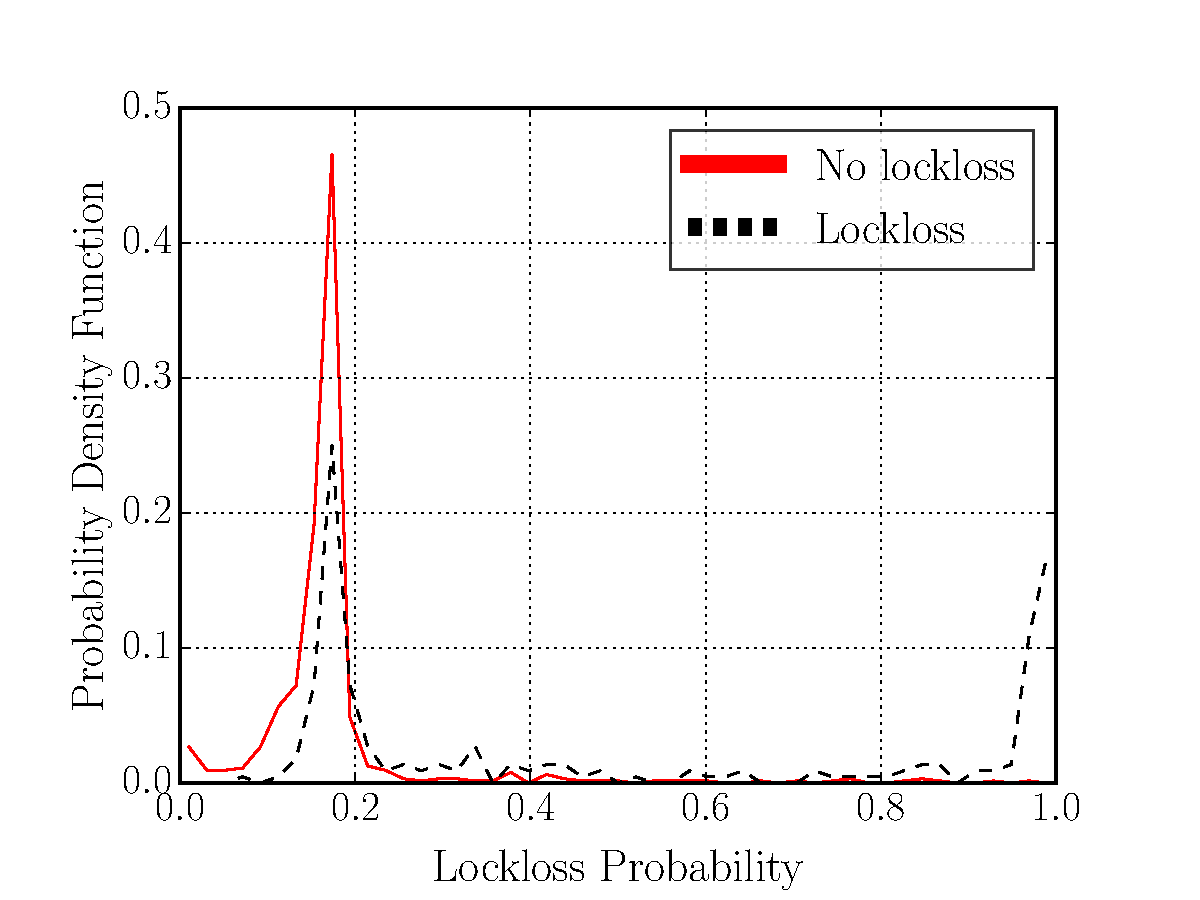
\includegraphics[width=3.5in,trim = 2.5cm 1.5cm 2.5cm 1.5cm, clip=true]{lockloss_histogram_H1O1O2_GPR.pdf}
 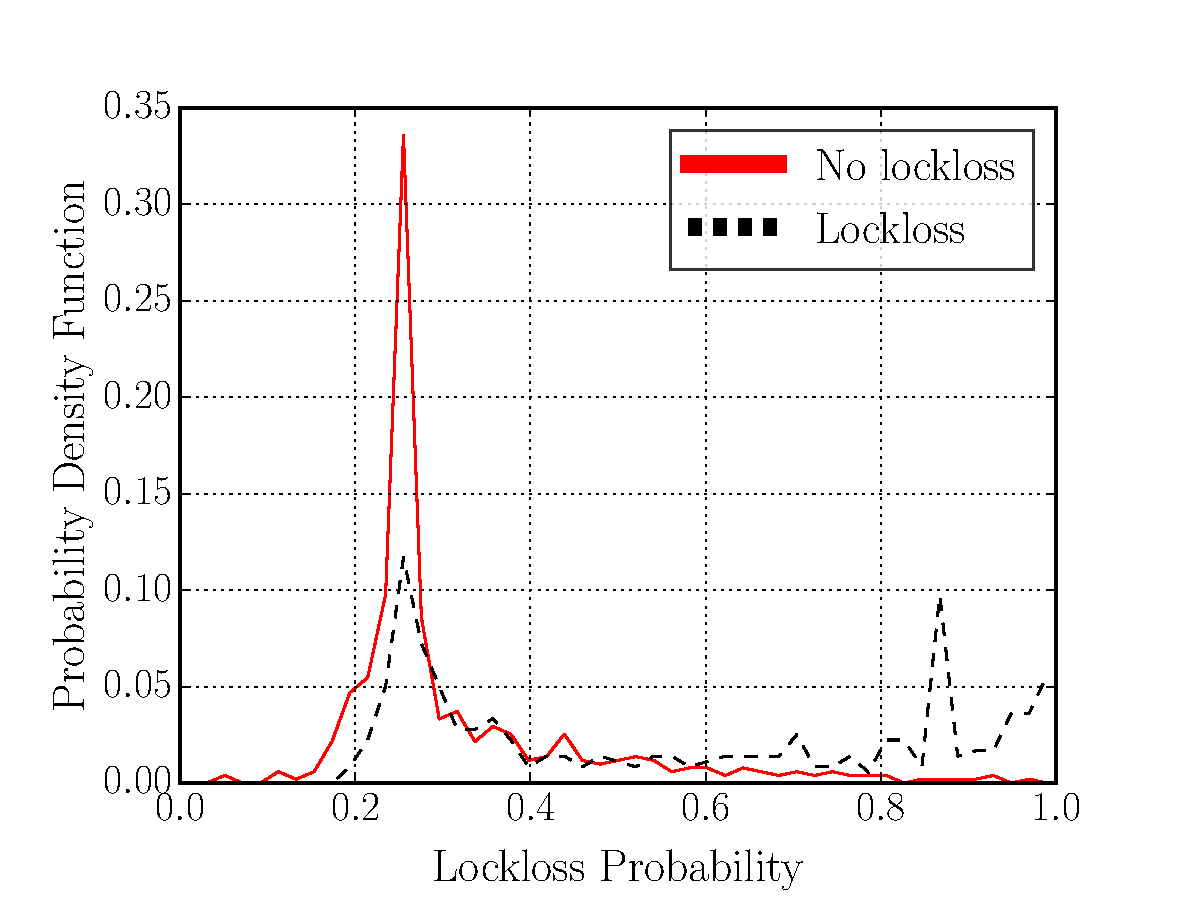
\includegraphics[width=3.5in,trim = 2.5cm 1.5cm 2.5cm 1.5cm, clip=true]{lockloss_histogram_L1O1O2_GPR.pdf}
 \caption{Histogram of lockloss probabilities predicted in O1-O2 at the interferometers (LHO and LLO) using Support Vector Machines.}
 \label{fig:lockloss}
\end{figure*}

It is useful to determine which earthquakes cause the loss of data and which will not affect the detector in a significant way.
In addition to the parameters that go into the ground velocity prediction model, we also use the prediction for the ground velocity to include when predicting the outcome of the interferometer lock status.
In previous work \cite{CoEa2017}, we found comparable performance among machine learning algorithms, and for this work use Support Vector Machines \cite{Burges_SVM}.
Figure~\ref{fig:lockloss} shows the distribution of the lockloss probabilities for O1 and O2 for both LHO and LLO. 

\section{Performance}
\label{sec:performance}

\section{Conclusion}
\label{sec:conclusions}


\section{Acknowledgments}
MC was supported by the National Science Foundation Graduate Research Fellowship
Program, under NSF grant number DGE 1144152. 
NM acknowledges Council for Scientific and Industrial Research (CSIR), India, for providing financial support as Senior Research Fellow.  
LIGO was constructed by the California Institute of Technology and Massachusetts Institute of Technology with funding from the National Science Foundation and operates under cooperative agreement PHY-0757058.
This paper has been assigned LIGO document number LIGO-P1600321.
The authors would like to thank Dr. Jenne Driggers for a detailed reading of an early version of the manuscript.

%\raggedright
\bibliographystyle{unsrt}
\bibliography{references}


\end{document} 
